238. \begin{figure}[ht!]
\center{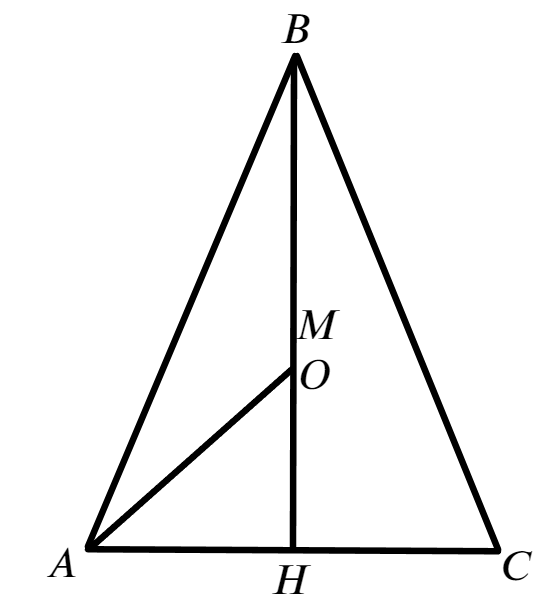
\includegraphics[scale=0.35]{g30-1.png}}
\end{figure}\\
Опустим высоту (она же биссектриса и медиана) $BH.$ Тогда $AH=HC=10:2=5,\ BH=\sqrt{13^2-5^2}=12,\ S_{\Delta ABC}=\cfrac{1}{2}\cdot12\cdot10=60.$ Так как $S_{\Delta ABC}=rp,$ а $p=\cfrac{13+13+10}{2}=18,$ имеем равенство $r=\cfrac{S_{\Delta ABC}}{p}=\cfrac{60}{18}=\cfrac{10}{3}.$ Так как медианы делятся точкой пересечения в отношении $2:1,$ считая от вершины, найдём $MH=\cfrac{1}{3}\cdot12=4,$ а $OH=r=\cfrac{10}{3},$ поэтому $MO=MH-OH=4-\cfrac{10}{3}=\cfrac{2}{3}.$\\
